\documentclass{article}
\usepackage[T1]{fontenc}
\usepackage{lmodern}
\usepackage{graphicx}
\usepackage{amsmath,amssymb}
\usepackage[a4paper,margin=2cm]{geometry}
\usepackage[absolute,overlay]{textpos}
\setlength{\TPHorizModule}{1mm}
\setlength{\TPVertModule}{1mm}
\usepackage[indonesian]{babel}
\usepackage{hyperref}
\setlength{\emergencystretch}{2em}
% unit: Halaman 114

\begin{document}

% === Halaman 114 (llm) ===

\begin{itemize}
    \item Posisi awal keempat \textit{rotor} dapat di-set; dan posisi awal ini menyatakan kunci dari Enigma.
    \item Kriptanalisis mesin Enigma pertama kali ditemukan pada tahun 1932 oleh kriptografer Polandia, yaitu Marian Rejewski, Jerzy Różycki dan Henryk Zygalski.
    \item Pemerintahan Nazi Jerman kemudian mendesain ulang mesin Enigma pada tahun 1939 dengan menambahkan \textbf{plugboard} dan \textbf{reflektor}, sehingga proses enkripsi menjadi lebih kompleks. Metode kriptanalisis Enigma sebelumnya tidak dapat digunakan lagi.
\end{itemize}

\vspace{44.55mm}

% deskripsi: Diagram skema kerja mesin Enigma yang menunjukkan aliran sinyal melalui Reflektor, Left Rotor, Middle Rotor, dan Right Rotor, mengilustrasikan proses enkripsi huruf A menjadi G dan A menjadi C.
% bbox normalisasi: [0.6050, 0.7500, 0.9900, 0.9000]
\begin{textblock*}{80.85mm}(127.05mm,222.75mm)
\noindent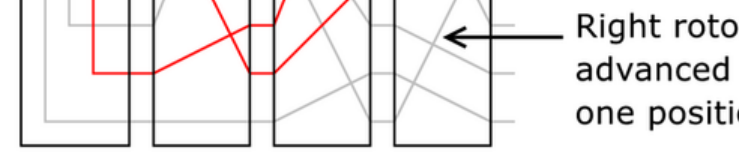
\includegraphics[width=80.85mm,height=44.55mm]{../../images/llm/page_114_img_01.png}%
\end{textblock*}

\end{document}
